\documentclass{article}

% Page layout
\usepackage{geometry}
\geometry{
	a4paper,
}

% Fonts
\usepackage{fontspec}
\defaultfontfeatures{Mapping=tex-text,Scale=MatchLowercase}
\setmainfont{Linux Libertine O}

% Language
\usepackage{polyglossia}
\setdefaultlanguage{english}

% Graphics
\usepackage{graphicx}
\graphicspath{{./images/}}

% Links
\usepackage{url,hyperref}

% Headers and footers
\usepackage{fancyhdr}
\pagestyle{fancy}
\fancyhf{}
\lhead{
\includegraphics[scale=0.4]{inp-enseeiht}}
\rhead{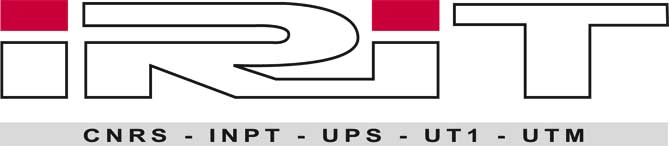
\includegraphics[scale=0.2]{irit}}
\lfoot{Three-dimensional modelling and printing}
\rfoot{\bfseries \thepage}

% Code
\usepackage{minted}

\begin{document}

\bigskip
\bigskip
\bigskip
\bigskip
\bigskip
\bigskip
\bigskip
\bigskip

\begin{center}
	\LARGE{Three-dimensional modelling and printing project:\\Set up documentation\\}
	\bigskip
	\bigskip
	\Large{from January 23 to March 16, 2012}
\end{center}

\bigskip
\bigskip

\begin{center}
\large{
\textit{Vincent \textsc{Duvert} \\
Antoine \textsc{Lubineau} \\
Caroline \textsc{Naud} \\
James \textsc{Packer} \\
Florian \textsc{Ribon}} \\
\bigskip
INP-ENSEEIHT/IMA 
}
\end{center}

\bigskip
\bigskip

	This report summarizes the context, organization, work and outcomes within the project 3D modeling and printing project suggested by the VORTEX team of IRIT to some of the third-year students in the IMA department of ENSEEIHT.

\bigskip
\bigskip

\begin{figure}[!h]
\begin{center}
	
\includegraphics[scale=0.4]{inp-enseeiht}
\end{center}
\end{figure}

\bigskip

\begin{center}
http://www.enseeiht.fr/fr/index.html \\
2 Rue Charles Camichel \\
31 071 TOULOUSE
\end{center}

\bigskip

\begin{figure}[!h]
\begin{center}
	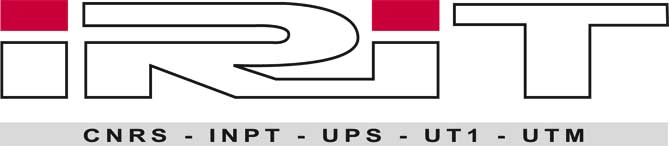
\includegraphics[scale=0.4]{irit}
\end{center}
\end{figure}

\begin{center}
http://www.info@irit.fr\\
Université Paul Sabatier \\
118 Route de Narbonne \\
F-31062 TOULOUSE CEDEX 9
\end{center}

\thispagestyle{empty}

\newpage

\tableofcontents

\newpage

\section{Global architecture of the application}

Here is (in orange) the different software and material you will have to get installed in order to use the complete application. The firmware is integrated in the printer and has not been modified in any way so you won't have to deal with it.

\begin{figure}[!h]
\begin{center}
	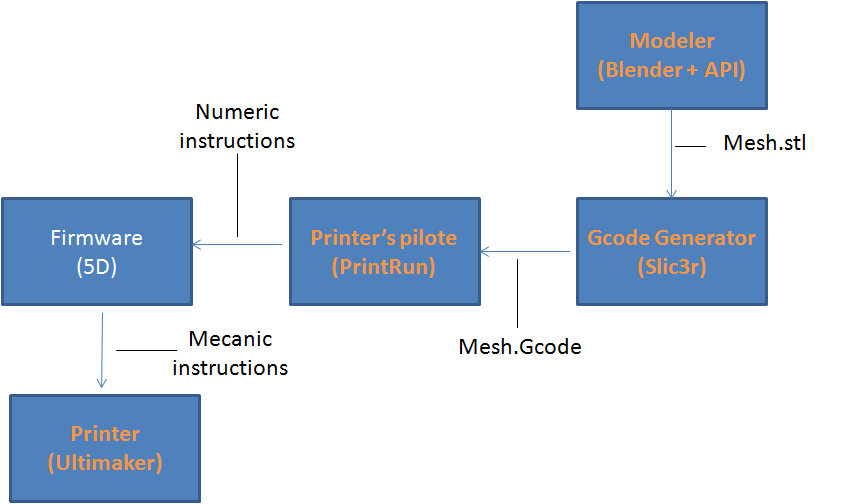
\includegraphics[scale=0.4]{ARD1}
\end{center}
\end{figure}

\section{Installing Blender}

\begin{description}
	\item[Homepage:] \url{http://www.blender.org/}
	\item[Recommended version:] \textbf{2.50 and older} because we use the Python 3 API, but scripts were only tested from versions 2.58 to 2.62.
\end{description}

\begin{description}
	\item[Windows] Download the latest version on \url{http://www.blender.org/download/get-blender/}.
	\item[Linux] Providing your distribution has a recent version of Blender, you should use your package manager. Else, you can download the 32~bits or 64~bits on \url{http://www.blender.org/download/get-blender/}.
	\item[MaxOS X] Go to \url{http://www.blender.org/download/get-blender/}.
\end{description}

\section{Installing Slic3r}

\begin{description}
	\item[Homepage:] \url{http://slic3r.org/}
	\item[Recommended version:] \textbf{0.7.0 and older}, as it provides cooling support, better mesh slicing, binary compatibility with Ubuntu 11.10, etc.
\end{description}

\begin{description}
	\item[Windows] Go to \url{http://dl.slic3r.org/win/} and download \texttt{slic3r-mswin-x86-0-7-0.zip}. Extract the file, and you can launch \texttt{slic3r.exe} from the \texttt{Slic3r} folder.
	\item[Linux] Go to \url{http://dl.slic3r.org/linux/} and download \texttt{slic3r-linux-x86-0-7-0.tar.gz}. To launch Slic3r:
		\begin{minted}{bash}
tar xz slic3r-linux-x86-0-7-0.tar.gz
cd Slic3r/bin
./slic3r
		\end{minted}
	\item[MaxOS X] Go to \url{http://dl.slic3r.org/mac/} and download \texttt{slic3r-osx-uni-0-7-0.dmg}.
\end{description}

\section{Installing Printrun}

\end{document}
